The rules mentioned (on lines 1, 4, 6, 9, 17, 22, 36–40, 42–44 and 49), without semantic actions (which make them all distinct), are:

\enumerate{
\item $reg  \rightarrow \langle Const\text{ } k \rangle$ (when fits move k)
\item $reg  \rightarrow \langle Local\text{ } n \rangle$ (when fits add n)
\item $reg  \rightarrow \langle Global\text{ } x \rangle$
\item $reg  \rightarrow \langle Loadw, addr \rangle$
\item $reg  \rightarrow \langle Binop\text{ } PlusA, reg1 , rand \rangle$
\item $reg  \rightarrow \langle Binop\text{ } Lsl, reg1, rand \rangle$
\item $rand \rightarrow \langle Const\text{ } k \rangle$ (when fits immed k)
\item $rand \rightarrow \langle Binop\text{ } Lsl, reg, \langle Const\text{ } n \rangle \rangle$ (when $n < 32$)
\item $rand \rightarrow \langle Binop\text{ } Lsl, reg1, reg2 \rangle$
\item $rand \rightarrow reg$
\item $addr \rightarrow \langle Local\text{ } n \rangle$ (when fits offset n)
\item $addr \rightarrow \langle Binop\text{ } PlusA, reg1, reg2 \rangle$
\item $addr \rightarrow \langle Binop\text{ } PlusA, reg1, \langle Binop\text{ } Lsl, reg2, \langle Const\text{ } n \rangle \rangle \rangle$ (when $n < 32$)
\item $addr \rightarrow reg$
\item $stmt \rightarrow \langle Storew, reg, addr \rangle$
}

\leavevmode
\\

Now to systematically calculate in how many ways we can tile the tree with these rules, we use dynamic programming:
\begin{itemize}
\item For each node $i$, and each symbol $S \in \{ stmt, addr, rand, reg \}$ we calculate $d_i^S$, the number of ways in which we can tile the subtree with it's root at $i$, and such that the tree can be generated from the symbol $S$, from bottom to top.
\item To find $d_i^S$, assuming that $d_j^\_$ has been found for all nodes $j \ne i$ in the subtree of $i$, use the following formula: \\
$d_i^S = \sum\limits_{\text{Pattern } p \text{ for } S \text { matches subtree at } i} (\prod\limits_{X \text{non-terminal in p}} d_{\text{node of } X}^X)$
\end{itemize}
\leavevmode
\par

The answer is in $d_{root}^{stmt}$. \\
\newpage
Numbering the nodes as in the diagram, the table holds synthesizes the information found by the dynamic programming algorithm:

\begin{minipage}[c]{.5\textwidth}
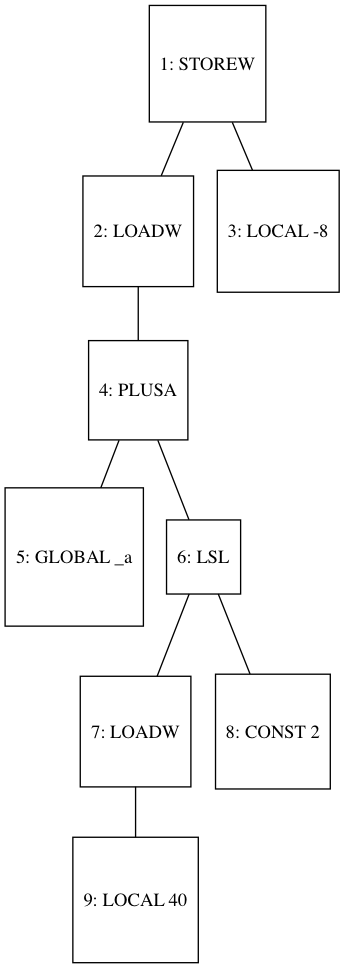
\includegraphics[width=.7\textwidth]{ex1.png}
\end{minipage}
\begin{minipage}[c]{.5\textwidth}
\begin{tabular}{|c|c|c|c|}

\hline
Node $i$ & Symbol $S$ & Rules & $d_i^S$ \\
\hline
1 & reg & & 0 \\
\hline
1 & rand & 10 & 0 \\
\hline
1 & addr & 14 & 0 \\
\hline
1 & stmt & 15 & \underline{28} \\
\hline

2 & reg & 4 & 14\\
\hline
2 & rand & 10 & 14\\
\hline
2 & addr & 14 & 14\\
\hline
2 & stmt & & 0 \\
\hline

3 & reg & 2 & 1\\
\hline
3 & rand & 10 & 1\\
\hline
3 & addr & 11, 14 & 2\\
\hline
3 & stmt & & 0 \\
\hline

4 & reg & 5 & 8\\
\hline
4 & rand & 10 & 8\\
\hline
4 & addr & 12, 13, 14& 14 \\
\hline
4 & stmt & & 0 \\

\hline
5 & reg & 3 & 1\\
\hline
5 & rand & 10 & 1\\
\hline
5 & addr & 14 & 1\\
\hline
5 & stmt & & 0 \\
\hline

6 & reg & 6 & 4\\
\hline
6 & rand & 8, 9, 10& 8\\
\hline
6 & addr & 14 & 4 \\
\hline
6 & stmt & & 0 \\
\hline

7 & reg & 4 & 2 \\
\hline
7 & rand & 10 & 2 \\
\hline
7 & addr & 14 & 2 \\
\hline
7 & stmt & & 0 \\
\hline

8 & reg & 1 & 1 \\
\hline
8 & rand & 7, 10 & 2 \\
\hline
8 & addr & 14 & 1\\
\hline
8 & stmt & & 0 \\
\hline

9 & reg & 2 & 1 \\
\hline
9 & rand & 10 & 1 \\
\hline
9 & addr & 11, 14& 2\\
\hline
9 & stmt & & 0 \\
\hline
\end{tabular}
\end{minipage}
So the answer is that there are 28 different tilings. \\

By inspecting all 28 trees, I've found that the shortest code is precisely the one in the notes:

\begin{lstlisting}{language=arm}
ldr r0, =_a
ldr r1, [fp, #40]
lsl r1, r1, #2
ldr r0, [r0, r1]
str r0, [fp, #-8]
\end{lstlisting}

And that the worst code is the one that uses the least specific rule at each possible choice (i.e. splits each node into its own tile), and that stores all temporary values in registers:

\begin{lstlisting}{language=arm}
ldr r0, [fp, #40]
ldr r1, [r0]
mov r2, #2
lsl r3, r1, r2
ldr r4, =_a
add r4, r4, r3
ldr r5, [r4]
ldr r6, [fp, #-8]
str r6, r0
\end{lstlisting}

This is almost the "bad" code from the notes, just that instead of directly computing \texttt{lsl r3, r1, \#2}, we first move \texttt{\#2} into a register and then compute this.
